\documentclass[tikz,border=3pt]{standalone}
\usepackage{amsmath,amssymb}
\usetikzlibrary{arrows.meta,calc,positioning}
\definecolor{ink}{HTML}{203344}
\definecolor{blue}{HTML}{286389}
\definecolor{teal}{HTML}{147D80}
\definecolor{gold}{HTML}{A36A20}
\definecolor{muted}{HTML}{596873}
\begin{document}
% Native 17.2 cm artwork: approximately 8 pt labels at ACL text width.
% Waveforms and feature tiles are schematic, not measured activations.
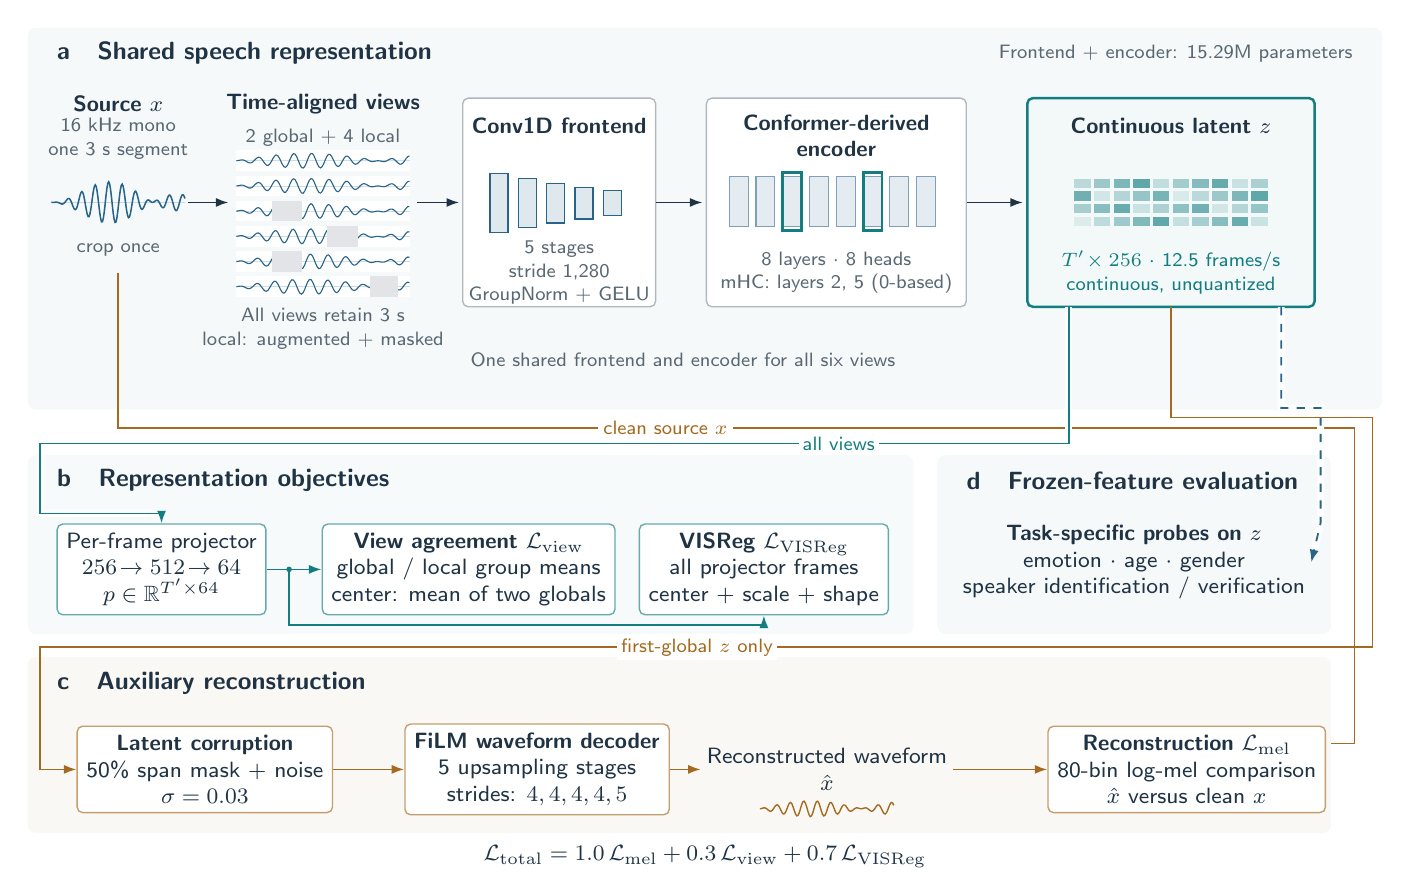
\begin{tikzpicture}[x=1cm,y=1cm,font=\sffamily\fontsize{8}{9.5}\selectfont,text=ink,
 flow/.style={-{Latex[length=1.6mm,width=1.15mm]},line width=.65pt,draw=ink},
 train/.style={flow,draw=teal},
 recon/.style={flow,draw=gold},
 eval/.style={flow,dashed,draw=blue},
 small/.style={font=\sffamily\fontsize{7}{8.5}\selectfont,text=muted},
 head/.style={font=\sffamily\bfseries\fontsize{9}{11}\selectfont,anchor=west},
 box/.style={rounded corners=2pt,draw=ink!35,fill=white,line width=.5pt,align=center},
 note/.style={align=center,inner sep=2pt}]
\path[use as bounding box] (0,0) rectangle (17.2,10.65);
% Panel A: aligned views and shared feature extraction.
\fill[blue!4,rounded corners=3pt] (0,5.8) rectangle (17.2,10.65);
\node[head] at (.25,10.32) {a\quad Shared speech representation};
\node[small,anchor=east] at (16.95,10.32) {Frontend + encoder: 15.29M parameters};
\node[note,font=\sffamily\bfseries\fontsize{8}{9.5}\selectfont] at (1.15,9.68) {Source $x$};
\node[small,note] at (1.15,9.24) {16 kHz mono\\one 3 s segment};
\draw[blue!25] (.3,8.43)--(2,8.43);
\draw[blue,line width=.55pt] plot[domain=0:1.7,samples=150] ({.3+\x},{8.43+.29*sin(\x*2100)*sin(\x*140)*sin(\x*93)});
\node[small] at (1.15,7.82) {crop once};
\draw[flow] (2.04,8.43)--(2.55,8.43);
\node[font=\sffamily\bfseries\fontsize{8}{9.5}\selectfont] at (3.75,9.68) {Time-aligned views};
\node[small] at (3.75,9.25) {2 global + 4 local};
\foreach \j in {0,...,5}{
 \pgfmathsetmacro{\yy}{8.96-\j*.32}
 \fill[white] (2.65,\yy-.13) rectangle (4.85,\yy+.13);
 \draw[blue!22,line width=.25pt] (2.65,\yy)--(4.85,\yy);
 \draw[blue,line width=.4pt] plot[domain=0:2.2,samples=110] ({2.65+\x},{\yy+.095*sin(\x*1600+\j*6)*sin(\x*100)});
}
\foreach \j/\a/\b in {2/3.1/3.48,3/3.8/4.2,4/3.1/3.48,5/4.35/4.7}{
 \pgfmathsetmacro{\yy}{8.96-\j*.32}
 \fill[ink!13] (\a,\yy-.13) rectangle (\b,\yy+.13);
}
\node[small,note] at (3.75,6.83) {All views retain 3 s\\local: augmented + masked};
\draw[flow] (4.95,8.43)--(5.48,8.43);
\node[box,minimum width=2.45cm,minimum height=2.65cm] (front) at (6.75,8.43) {};
\node[font=\sffamily\bfseries\fontsize{8}{9.5}\selectfont] at (6.75,9.4) {Conv1D frontend};
\foreach \i/\h in {0/.75,1/.62,2/.5,3/.4,4/.32}{
 \filldraw[fill=blue!15,draw=blue,line width=.45pt] ({5.87+\i*.36},{8.42-\h/2}) rectangle ++(.23,\h);
}
\node[small,note] at (6.75,7.54) {5 stages\\stride 1,280\\GroupNorm + GELU};
\draw[flow] (front.east)--(8.57,8.43);
\node[box,minimum width=3.3cm,minimum height=2.65cm] (enc) at (10.27,8.43) {};
\node[align=center,font=\sffamily\bfseries\fontsize{8}{9.5}\selectfont] at (10.27,9.28) {Conformer-derived\\encoder};
\foreach \i in {0,...,7}{
 \filldraw[fill=blue!12,draw=blue!60,line width=.4pt] ({8.91+\i*.34},8.12) rectangle ++(.24,.64);
}
\foreach \i in {2,5}{
 \draw[teal,line width=1pt] ({8.91+\i*.34},8.07) rectangle ++(.24,.74);
}
\node[small,note] at (10.27,7.54) {8 layers $\cdot$ 8 heads\\mHC: layers 2, 5 (0-based)};
\draw[flow] (enc.east)--(12.64,8.43);
\node[box,draw=teal,line width=.9pt,fill=teal!5,minimum width=3.65cm,minimum height=2.65cm] (z) at (14.52,8.43) {};
\node[font=\sffamily\bfseries\fontsize{8}{9.5}\selectfont] at (14.52,9.4) {Continuous latent $z$};
\foreach \i in {0,...,9}{\foreach \j in {0,...,3}{
 \pgfmathtruncatemacro{\shade}{15+mod(\i*13+\j*23,55)}
 \fill[teal!\shade] ({13.29+\i*.25},{8.13+\j*.16}) rectangle ++(.21,.12);
}}
\node[small,note,text=teal] at (14.52,7.54) {$T'\!\times256$ $\cdot$ 12.5 frames/s\\continuous, unquantized};
\node[small,anchor=west] at (5.5,6.43) {One shared frontend and encoder for all six views};
% Clean target is an independent routed source branch.
\draw[recon] (1.15,7.54)--(1.15,5.57)--(16.85,5.57)--(16.85,1.56)--(16.36,1.56);
\node[small,text=gold,fill=white,inner sep=2pt] at (8.1,5.57) {clean source $x$};
% Panel B: projector-space regularization, plus evaluation.
\fill[teal!4,rounded corners=3pt] (0,2.95) rectangle (11.25,5.22);
\node[head] at (.25,4.9) {b\quad Representation objectives};
\node[box,draw=teal!65,minimum width=2.5cm,minimum height=1.15cm] (proj) at (1.7,3.77) {Per-frame projector\\$256\!\rightarrow512\!\rightarrow64$\\$p\in\mathbb{R}^{T'\times64}$};
\node[box,draw=teal!65,minimum width=3.3cm,minimum height=1.15cm] (view) at (5.6,3.77) {\textbf{View agreement} $\mathcal L_{\mathrm{view}}$\\global / local group means\\center: mean of two globals};
\node[box,draw=teal!65,minimum width=3.15cm,minimum height=1.15cm] (vis) at (9.35,3.77) {\textbf{VISReg} $\mathcal L_{\mathrm{VISReg}}$\\all projector frames\\center + scale + shape};
% Routed z branches in the whitespace between panels.
\draw[train,preaction={draw=white,line width=2.5pt}] (13.22,7.1)--(13.22,5.37)--(.16,5.37)--(.16,4.48)--(1.7,4.48)--(proj.north);
\node[small,text=teal,fill=white,inner sep=1.5pt] at (10.3,5.37) {all views};
\draw[train] (proj.east)--(view.west);
\draw[train] (3.32,3.77)--(3.32,3.06)--(9.35,3.06)--(vis.south);
\fill[teal] (3.32,3.77) circle (1pt);
\fill[blue!4,rounded corners=3pt] (11.55,2.95) rectangle (16.55,5.22);
\node[head] at (11.8,4.9) {d\quad Frozen-feature evaluation};
\node[note] (probe) at (14.05,3.86) {\textbf{Task-specific probes on $z$}\\emotion $\cdot$ age $\cdot$ gender\\speaker identification / verification};
\draw[eval,preaction={draw=white,line width=2.5pt}] (15.92,7.1)--(15.92,5.82)--(16.42,5.82)--(16.42,4.36)--(probe.east);
% Panel C: reconstruction, kept wholly in z-space.
\fill[gold!5,rounded corners=3pt] (0,.42) rectangle (16.55,2.66);
\node[head] at (.25,2.33) {c\quad Auxiliary reconstruction};
\node[box,draw=gold!65,minimum width=3.2cm,minimum height=1.02cm] (corrupt) at (2.25,1.23) {\textbf{Latent corruption}\\50\% span mask + noise\\$\sigma=0.03$};
\node[box,draw=gold!65,minimum width=3.2cm,minimum height=1.02cm] (decoder) at (6.47,1.23) {\textbf{FiLM waveform decoder}\\5 upsampling stages\\strides: $4,4,4,4,5$};
\node[note] (out) at (10.15,1.23) {Reconstructed waveform\\$\hat{x}$};
\draw[gold,line width=.5pt] plot[domain=0:1.7,samples=110] ({9.3+\x},{.73+.10*sin(\x*2100)*sin(\x*140)});
\node[box,draw=gold!65,minimum width=3.2cm,minimum height=1.02cm] (mel) at (14.72,1.23) {\textbf{Reconstruction} $\mathcal L_{\mathrm{mel}}$\\80-bin log-mel comparison\\$\hat{x}$ versus clean $x$};
\draw[recon] (14.52,7.1)--(14.52,5.7)--(17.08,5.7)--(17.08,2.78)--(.16,2.78)--(.16,1.23)--(corrupt.west);
\node[small,text=gold,fill=white,inner sep=1.5pt] at (8.5,2.78) {first-global $z$ only};
\draw[recon] (corrupt.east)--(decoder.west);
\draw[recon] (decoder.east)--(out.west);
\draw[recon] (out.east)--(mel.west);
\node[font=\sffamily\fontsize{8}{10}\selectfont] at (8.6,.12) {$\mathcal L_{\mathrm{total}}=1.0\,\mathcal L_{\mathrm{mel}}+0.3\,\mathcal L_{\mathrm{view}}+0.7\,\mathcal L_{\mathrm{VISReg}}$};
\end{tikzpicture}
\end{document}
